% (find-LATEX "2020-2-C3-rcadeia1.tex")
% (defun c () (interactive) (find-LATEXsh "lualatex -record 2020-2-C3-rcadeia1.tex" :end))
% (defun C () (interactive) (find-LATEXsh "lualatex 2020-2-C3-rcadeia1.tex" "Success!!!"))
% (defun D () (interactive) (find-pdf-page      "~/LATEX/2020-2-C3-rcadeia1.pdf"))
% (defun d () (interactive) (find-pdftools-page "~/LATEX/2020-2-C3-rcadeia1.pdf"))
% (defun e () (interactive) (find-LATEX "2020-2-C3-rcadeia1.tex"))
% (defun o () (interactive) (find-LATEX "2020-2-C3-rcadeia1.tex"))
% (defun u () (interactive) (find-latex-upload-links "2020-2-C3-rcadeia1"))
% (defun v () (interactive) (find-2a '(e) '(d)))
% (defun d0 () (interactive) (find-ebuffer "2020-2-C3-rcadeia1.pdf"))
% (defun cv () (interactive) (C) (ee-kill-this-buffer) (v) (g))
%          (code-eec-LATEX "2020-2-C3-rcadeia1")
% (find-pdf-page   "~/LATEX/2020-2-C3-rcadeia1.pdf")
% (find-sh0 "cp -v  ~/LATEX/2020-2-C3-rcadeia1.pdf /tmp/")
% (find-sh0 "cp -v  ~/LATEX/2020-2-C3-rcadeia1.pdf /tmp/pen/")
%     (find-xournalpp "/tmp/2020-2-C3-rcadeia1.pdf")
%   file:///home/edrx/LATEX/2020-2-C3-rcadeia1.pdf
%               file:///tmp/2020-2-C3-rcadeia1.pdf
%           file:///tmp/pen/2020-2-C3-rcadeia1.pdf
% http://angg.twu.net/LATEX/2020-2-C3-rcadeia1.pdf
% (find-LATEX "2019.mk")
% (find-CN-aula-links "2020-2-C3-rcadeia1" "3" "c3m202rcadeia1" "c37")
%
% Video:
% (find-ssr-links     "c3m202rcadeia1" "2020-2-C3-rcadeia1" "{hash}")
% (code-eevvideo      "c3m202rcadeia1" "2020-2-C3-rcadeia1" "{hash}")
% (code-eevlinksvideo "c3m202rcadeia1" "2020-2-C3-rcadeia1" "{hash}")
% (find-c3m202rcadeia1video "0:00")

% «video-numerozinhos»  (to ".video-numerozinhos")
% (c3m202rcadeia1a "video-numerozinhos")
% (find-ssr-links     "c3m202rcadeia1b" "2020-2-C3-rcadeia1-b" "{hash}")
% (code-eevvideo      "c3m202rcadeia1b" "2020-2-C3-rcadeia1-b" "{hash}")
% (code-eevlinksvideo "c3m202rcadeia1b" "2020-2-C3-rcadeia1-b" "{hash}")
% (find-c3m202rcadeia1bvideo "0:00")
% (find-c3m202rcadeia1bvideo "0:48" "Exercicio 4")
% (find-c3m202rcadeia1bvideo "1:11" "vão ter que ver como o Bortolossi desenha")
% (find-c3m202rcadeia1bvideo "1:52" "ele tem alguns truques de visualização")
% (find-c3m202rcadeia1bvideo "2:11" "pontos em R^3 em perspectiva")
% (find-c3m202rcadeia1bvideo "2:30" "e aí explica como fazer cortes")
% (find-c3m202rcadeia1bvideo "2:45" "cortes em planos paralelos ao plano xy")
% (find-c3m202rcadeia1bvideo "3:25" "cortes em outros planos")
% (find-c3m202rcadeia1bvideo "4:25" "ruim porque tem raízes quadradas")
% (find-c3m202rcadeia1bvideo "5:10" "G(x,y) = x^2+y^2")
% (find-c3m202rcadeia1bvideo "6:54" "G(0,0) = 0, G(1,0) = ...")
% (find-c3m202rcadeia1bvideo "7:53" "e agora a gente vai desenhar eles no plano")
% (find-c3m202rcadeia1bvideo "8:05" "em cima do ponto (0,0)")

% (find-ssr-links     "c3m202rcadeia1c" "2020-2-C3-rcadeia1-c" "{hash}")
% (code-eevvideo      "c3m202rcadeia1c" "2020-2-C3-rcadeia1-c" "{hash}")
% (code-eevlinksvideo "c3m202rcadeia1c" "2020-2-C3-rcadeia1-c" "{hash}")
% (find-c3m202rcadeia1cvideo "0:00")
% (find-c3m202rcadeia1cvideo "3:34" "é o ponto que tem z=1")
% (find-c3m202rcadeia1cvideo "5:42" "")

% (find-ssr-links     "c3m202rcadeia1d" "2020-2-C3-rcadeia1-d" "{hash}")
% (code-eevvideo      "c3m202rcadeia1d" "2020-2-C3-rcadeia1-d" "{hash}")
% (code-eevlinksvideo "c3m202rcadeia1d" "2020-2-C3-rcadeia1-d" "{hash}")
% (find-c3m202rcadeia1dvideo "0:00")

% 2021mar26
% (find-ssr-links     "c3m202rcadeia1e" "2020-2-C3-rcadeia1-e" "{hash}")
% (code-eevvideo      "c3m202rcadeia1e" "2020-2-C3-rcadeia1-e" "{hash}")
% (code-eevlinksvideo "c3m202rcadeia1e" "2020-2-C3-rcadeia1-e" "{hash}")
% (find-c3m202rcadeia1evideo "0:00")
% (find-c3m202rcadeia1evideo "0:40" "Uma figura do livro do Thomas")
% (find-c3m202rcadeia1evideo "6:50" "Delta x")
% (find-c3m202rcadeia1evideo "11:35" "é o meu ponto (x_0,y_0)")

% «.video-numerozinhos»	(to "video-numerozinhos")
%
% «.defs»		(to "defs")
% «.title»		(to "title")
% «.exercicio-1»	(to "exercicio-1")
% «.exercicio-1-dica»	(to "exercicio-1-dica")
% «.exercicio-2»	(to "exercicio-2")
% «.tipos»		(to "tipos")
% «.exercicio-3»	(to "exercicio-3")
% «.semi-esfera»	(to "semi-esfera")
% «.exercicio-4»	(to "exercicio-4")
% «.exercicio-5»	(to "exercicio-5")
% «.exercicio-6»	(to "exercicio-6")
% «.exercicio-7»	(to "exercicio-7")
% «.exercicio-8»	(to "exercicio-8")
% «.exercicio-9»	(to "exercicio-9")
% «.exercicio-9-dicas»	(to "exercicio-9-dicas")
% «.dicas-sobre-as-dicas»	(to "dicas-sobre-as-dicas")
% «.thomas-intro»	(to "thomas-intro")
% «.figura-thomas»	(to "figura-thomas")
% «.exercicio-10»	(to "exercicio-10")
% «.tipos-de-novo»	(to "tipos-de-novo")
% «.exercicio-13»	(to "exercicio-13")
% «.exercicio-14»	(to "exercicio-14")
% «.exercicio-15»	(to "exercicio-15")
%
% «.djvuize»	(to "djvuize")

\documentclass[oneside,12pt]{article}
\usepackage[colorlinks,citecolor=DarkRed,urlcolor=DarkRed]{hyperref} % (find-es "tex" "hyperref")
\usepackage{amsmath}
\usepackage{amsfonts}
\usepackage{amssymb}
\usepackage{pict2e}
\usepackage[x11names,svgnames]{xcolor} % (find-es "tex" "xcolor")
\usepackage{colorweb}                  % (find-es "tex" "colorweb")
%\usepackage{tikz}
%
% (find-dn6 "preamble6.lua" "preamble0")
\usepackage{proof}   % For derivation trees ("%:" lines)
\input diagxy        % For 2D diagrams ("%D" lines)
\xyoption{curve}     % For the ".curve=" feature in 2D diagrams
%
\usepackage{edrx15}               % (find-LATEX "edrx15.sty")
\input edrxaccents.tex            % (find-LATEX "edrxaccents.tex")
\input edrxchars.tex              % (find-LATEX "edrxchars.tex")
\input edrxheadfoot.tex           % (find-LATEX "edrxheadfoot.tex")
\input edrxgac2.tex               % (find-LATEX "edrxgac2.tex")
%
%\usepackage[backend=biber,
%   style=alphabetic]{biblatex}            % (find-es "tex" "biber")
%\addbibresource{catsem-slides.bib}        % (find-LATEX "catsem-slides.bib")
%
% (find-es "tex" "geometry")
\usepackage[a6paper, landscape,
            top=1.5cm, bottom=.25cm, left=1cm, right=1cm, includefoot
           ]{geometry}
%
\begin{document}

\catcode`\^^J=10
\directlua{dofile "dednat6load.lua"}  % (find-LATEX "dednat6load.lua")

% %L dofile "edrxtikz.lua"  -- (find-LATEX "edrxtikz.lua")
% %L dofile "edrxpict.lua"  -- (find-LATEX "edrxpict.lua")
% \pu

% «defs»  (to ".defs")
% (find-LATEX "edrx15.sty" "colors-2019")
\long\def\ColorRed   #1{{\color{Red1}#1}}
\long\def\ColorViolet#1{{\color{MagentaVioletLight}#1}}
\long\def\ColorViolet#1{{\color{Violet!50!black}#1}}
\long\def\ColorGreen #1{{\color{SpringDarkHard}#1}}
\long\def\ColorGreen #1{{\color{SpringGreenDark}#1}}
\long\def\ColorGreen #1{{\color{SpringGreen4}#1}}
\long\def\ColorGray  #1{{\color{GrayLight}#1}}
\long\def\ColorGray  #1{{\color{black!30!white}#1}}
\long\def\ColorBrown #1{{\color{Brown}#1}}
\long\def\ColorBrown #1{{\color{brown}#1}}
\long\def\ColorOrange#1{{\color{orange}#1}}

\long\def\ColorShort #1{{\color{SpringGreen4}#1}}
\long\def\ColorLong  #1{{\color{Red1}#1}}

\def\frown{\ensuremath{{=}{(}}}
\def\True {\mathbf{V}}
\def\False{\mathbf{F}}
\def\D    {\displaystyle}

\def\drafturl{http://angg.twu.net/LATEX/2020-2-C3.pdf}
\def\drafturl{http://angg.twu.net/2020.2-C3.html}
\def\draftfooter{\tiny \href{\drafturl}{\jobname{}} \ColorBrown{\shorttoday{} \hours}}



%  _____ _ _   _                               
% |_   _(_) |_| | ___   _ __   __ _  __ _  ___ 
%   | | | | __| |/ _ \ | '_ \ / _` |/ _` |/ _ \
%   | | | | |_| |  __/ | |_) | (_| | (_| |  __/
%   |_| |_|\__|_|\___| | .__/ \__,_|\__, |\___|
%                      |_|          |___/      
%
% «title»  (to ".title")
% (c3m202rcadeia1p 1 "title")
% (c3m202rcadeia1a   "title")

\thispagestyle{empty}

\begin{center}

\vspace*{1.2cm}

{\bf \Large Cálculo 3 - 2020.2}

\bsk

Aula 7: Regra da Cadeia (1)

(E um pouco de curvas de nível)

\bsk

Eduardo Ochs - RCN/PURO/UFF

\url{http://angg.twu.net/2020.2-C3.html}

\end{center}

\newpage

% «exercicio-1»  (to ".exercicio-1")
% (c3m202rcadeia1p 2 "exercicio-1")
% (c3m202rcadeia1a   "exercicio-1")

% (find-bortolossi5page (+ -162 172) "omitir os pontos onde as parciais são calculadas")

Dê uma olhada nas páginas 172 e 173 do capítulo 5 do Bortolossi, onde
ele diz ``Cuidado! Cuidado! Cuidado!''... ele fala que vai evitar
certas notações. Nos exercícios de hoje nós vamos começar a usar
algumas das notações que ele prefere evitar, e daqui a algumas aulas
nós vamos aprender a formalizar essas notações.

\bsk

{\bf Exercício 1.}

Seja $h(x) = f(g(x))$.

Sabemos que $h'(x) = f'(g(x)) g'(x)$, pela regra da cadeia...

a) Calcule $h''(x)$.

b) Calcule $h'''(x)$.

\bsk

Dica: 
%
% (find-latexscan-links "C3" "20210226_regra_da_cadeia_1")
% (find-xpdf-page "~/LATEX/2020-2-C3/20210226_regra_da_cadeia_1.pdf")
$\myvcenter{
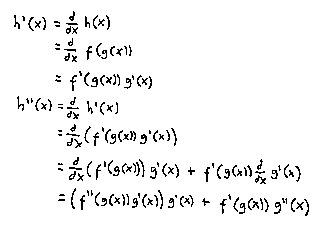
\includegraphics[height=2cm]{2020-2-C3/20210226_regra_da_cadeia_1.pdf}
}$

\newpage

{\bf Exercício 1 (cont.)}

\ssk

Repare que nos itens acima $g$, $g'$, $g''$ e $g'''$ sempre aparecem
``calculadas no ponto $x$'', ou seja, como $g(x)$, $g'(x)$, $g''(x)$ e
$g'''(x)$... e $f$, $f'$, $f''$ e $f'''$ sempre aparecem ``calculadas
no ponto $g(x)$'', ou seja, como $f(g(x))$, $f'(g(x))$, $f''(g(x))$ e
$f'''(g(x))$. Se abreviarmos as nossas contas omitindo esses pontos de
aplicação vamos conseguir fórmulas bem mais curtas, como $h'=f'g'$.

c) Reescreva $h''(x)$ usando essas abreviações. % $h''= \; \ColorRed{?}$

d) Reescreva $h'''(x)$ usando essas abreviações. % $h'''= \; \ColorRed{?}$



\newpage

% «exercicio-1-dica»  (to ".exercicio-1-dica")
% (c3m202rcadeia1p 4 "exercicio-1-dica")
% (c3m202rcadeia1a   "exercicio-1-dica")

Dica:

\bsk

%D diagram ex1-dica1
%D 2Dx     100 +70 +55
%D 2D  100 A0
%D 2D
%D 2D  +20 B0
%D 2D
%D 2D  +20 C0  C1
%D 2D
%D 2D  +20 D0  D1  D2
%D 2D
%D ren A0 ==> f(g(x))
%D ren B0 ==> f'(g(x))g'(x)
%D ren C0 C1 ==> f''(g(x))g'(x)g'(x) f'(g(x))g''(x)
%D ren D0 D1 D2 ==> f'''(g(x))g'(x)g'(x)g'(x) f''(g(x))g'(x)g''(x)  f'(g(x))g'''(x)
%D
%D (( A0 B0 -> # A0 B1 ->
%D    B0 C0 -> B0 C1 -> # B1 C1 -> B1 C2 ->
%D    C0 D0 -> C0 D1 -> C1 D1 -> C1 D2 -> # C2 D2 -> C2 D3 ->
%D
%D ))
%D enddiagram
%D
%D diagram ex1-dica2
%D 2Dx     100 +30 +25
%D 2D  100 A0
%D 2D
%D 2D  +20 B0
%D 2D
%D 2D  +20 C0  C1
%D 2D
%D 2D  +20 D0  D1  D2
%D 2D
%D ren A0 ==> f
%D ren B0 ==> f'g'
%D ren C0 C1 ==> f''g'g' f'g''
%D ren D0 D1 D2 ==> f'''g'g'g' f''g'g'' f'g'''
%D
%D (( A0 B0 -> # A0 B1 ->
%D    B0 C0 -> B0 C1 -> # B1 C1 -> B1 C2 ->
%D    C0 D0 -> C0 D1 -> C1 D1 -> C1 D2 -> # C2 D2 -> C2 D3 ->
%D
%D ))
%D enddiagram
%D
$\pu
  \scalebox{0.70}{$
  \diag{ex1-dica1}
  \qquad
  \diag{ex1-dica2}
  $}
$

\bsk
\bsk

% Exemplo:

$$\begin{array}{l}
  \frac{d}{dx} \; f''(g(x))g'(x)g'(x) \\
  = \; f'''(g(x))g'(x)g'(x)g'(x) + 2 f''(g(x))g'(x)g''(x) \\
  \end{array}
$$


\newpage

Agora nós vamos começar a ver funções de $\R^2$ em $\R$, que vão
definir \ColorRed{superfícies}. Por exemplo, se $F(x,y) = x^2+y^2$
então este conjunto
%
$$\setofxyzst{z = F(x,y)}$$

vai ser uma superfície --- um parabolóide.

Nos outros semestres eu tentei ensinar superfícies começando por um
método de ``ligue os pontos'' em 3D, que era uma adaptação da idéia de
que podemos desenhar uma aproximação para um curva em $\R^2$ começando
pelos pontos $(a-1,f(a-1))$, $(a,f(a))$, $(a+1,f(a+1))$...

\newpage

...mas desta vez nós vamos começar por dois outros assuntos:

\begin{itemize}

\item Cortes. \ColorRed{Dê uma olhada no capítulo 3 do Bortolossi, nas
  páginas 81 até 95. Tente pelo menos entender as figuras!}

% (find-bortolossi3page (+ -78  81) "3.2. Funções de duas variáveis")
% (find-bortolossi3page (+ -78  86)   "Vamos tentar outros cortes. (Figs: pp.90-95)")
% (find-bortolossi3page (+ -78  93)   "Exemplo 3.2. Sela de cavalo.")

\item Derivadas parciais. \ColorRed{Dê uma olhada no capítulo 5 do
  Bortolossi, nas páginas 163 até 167. Tente pelo menos entender as
  figuras!} Os próximos exercícios vão nos ajudar a entender estas
  idéias na prática.

% (find-bortolossi5page (+ -161 162) "5. Derivadas parciais")
% (find-bortolossi5page (+ -161 162) "5.1. Lembrando Cálculo 1")
% (find-bortolossi5page (+ -162 164) "5.2. Definições e exemplos")
% (find-bortolossi5page (+ -162 165)   "Fig. 5.2: Interpretação geométrica")
% (find-bortolossi5page (+ -162 167)   "Exemplo 5.1: Cobb-Douglas")
% (find-bortolossi5page (+ -162 170)   "derivada parcial")
% (find-bortolossi5page (+ -162 171)   "a notação D_1 f é a mais clara")
% (find-bortolossi5page (+ -162 172)   "omitir os pontos onde as parciais são calculadas")

\end{itemize}


\newpage

% «exercicio-2»  (to ".exercicio-2")
% (c3m202rcadeia1p 7 "exercicio-2")
% (c3m202rcadeia1a   "exercicio-2")

{\bf Exercício 2.}

\ssk

Sejam $F(x,y) = (x+5)y$, $g(t) = \sen t$, $h(t) = e^{2t}$.

a) Calcule $\frac{d}{dt} F(g(t),h(t))$.

b) Calcule $\frac{∂}{∂x}F(x,y)$ e $\frac{∂}{∂y}F(x,y)$.

c) Calcule $\frac{d}{dt}g(t)$ e $\frac{d}{dt}h(t)$.

\msk

Nós vamos usar bastante as notações $F_x = \frac{∂}{∂x}F$ e $F_y =
\frac{∂}{∂y}F$,

que o Bortolossi usa pouco.

d) Calcule $F_x(x,y)$ e $F_y(x,y)$.

e) Calcule $F_x(g(t),h(t))g'(t)$ e $F_y(g(t),h(t))h'(t)$.

A (e) deve dar o mesmo resultado que a (a).

\msk

Faça todos os itens do exercício [01] da página 177

do Bortolossi (no capítulo 5).


\newpage

% «tipos»  (to ".tipos")
% (c3m202rcadeia1p 8 "tipos")
% (c3m202rcadeia1a   "tipos")

{\bf Tipos}

\ssk

{\bf TUDO} que nós vamos fazer em Cálculo 3 pode ser {\sl visualizado}
e {\sl tipado}. Você já viu um pouco de tipos em {\tt C} e em Física;
em Física os ``tipos'' são parcialmente determinados pelas unidades
--- metros são distância, segundos são tempo, metros/segundo é uma
unidade de velocidade, e assim por diante...

Dê uma olhada nas páginas 164 a 166 do capítulo 5 do Bortolossi. Todas
as expressões que aparecem lá podem ser ``tipadas'' e interpretadas
como posições no eixo $x$ (ou no eixo $y$, ou no eixo $y$), ou como
distâncias no eixo $x$ (ou no eixo $y$, ou $z$), ou como {\sl
  inclinações}... vamos ver os detalhes disto aos poucos.

\newpage

Além das abreviações que nós vimos nos slides anteriores, em que a
gente só omite o ponto de avaliação e escreve ``$g$'' ao invés de
``$g(t)$'', existe uma outra convenção de abreviações que enfatiza os
``tipos'': a ``notação de Leibniz''. Por exemplo, se a gente
\ColorRed{define} que
%
$$\begin{array}{rcl}
  x = g(t) \\
  y = h(t) \\
  z = F(x,y) \\
  \end{array}
$$
%
então $z=F(g(t),h(t))$, $z_x = F_x(g(t),h(t))$, etc.

\newpage

% «exercicio-3»  (to ".exercicio-3")

{\bf Exercício 3.}

\ssk

a) Digamos que $y = g(x)$ e $z = f(y)$. Traduza isto aqui para notação
padrão: $\frac{dz}{dy} \frac{dy}{dx} = \frac{dz}{dx}$.

b) Digamos que $y = g(x)$ e $z = f(y)$. Calcule $z_{xx}$ de dois
jeitos: à esquerda use a notação de Leibniz, à direita traduza todas
as suas contas da esquerda para notação padrão.

c) Digamos que $x = g(t)$, $y = h(t)$, $z = F(x,y)$. Traduza isto aqui
para notação padrão: $\frac{dz}{dt} = z_x x_t + z_y y_t$. Faça a
tradução bem passo a passo se precisar!

d) Calcule $\frac{d}{dt} \frac{d}{dt} z$ e traduza as suas contas para
a notação padrão.




\newpage

% «semi-esfera»  (to ".semi-esfera")
% (c3m202rcadeia1p 11 "semi-esfera")
% (c3m202rcadeia1a    "semi-esfera")

Agora vamos fazer uma série de exercícios que têm a ver com os
``cortes'' que o Bortolossi explica nas páginas 81 a 95 (no capítulo
3). Seja $F(x,y)$ esta função aqui:
%
$$ F(x,y) =
\begin{cases}
  \sqrt{5^2 - x^2 - y^2} & \text{quando $5^2 - x^2 - y^2≥0$}, \\
  0 & \text{quando $5^2 - x^2 - y^2<0$,} \\
 \end{cases}
$$

% (find-bortolossi3page (+ -78  81) "3.2. Funções de duas variáveis")
% (find-bortolossi3page (+ -78  86)   "Vamos tentar outros cortes. (Figs: pp.90-95)")
% (find-bortolossi3page (+ -78  93)   "Exemplo 3.2. Sela de cavalo.")

% «exercicio-4»  (to ".exercicio-4")
% (c3m202rcadeia1p 11 "exercicio-4")
% (c3m202rcadeia1a    "exercicio-4")

{\bf Exercício 4.}

\ssk

Represente graficamente estes subconjuntos de $\R^2$:

a) $\setofxyst{5^2 - x^2 - y^2 = 0}$

b) $\setofxyst{5^2 - x^2 - y^2 < 0}$

c) $\setofxyst{5^2 - x^2 - y^2 ≥ 0}$

d) $\setofxyst{F(x,y)=1}$

e) $\setofxyst{F(x,y)=2}$

f) $\setofxyst{F(x,y)=3}$

\newpage

{\bf Exercício 4 (cont.)}

\ssk

g) $\setofxyst{F(x,y)=4}$

h) $\setofxyst{F(x,y)=5}$

i) $\setofxyst{F(x,y)=6}$

j) $\setofxyst{F(x,y)=0}$

k) $\setofxyst{F(x,y)=-1}$

\newpage

% «exercicio-5»  (to ".exercicio-5")
% (c3m202rcadeia1p 13 "exercicio-5")
% (c3m202rcadeia1a    "exercicio-5")

{\bf Exercício 5.}

\ssk

Agora seja $S$ esta superfície ($S ⊆ \R^3$):
%
$$S = \setofxyzst{z = F(x,y)}.$$

Represente graficamente os seguintes cortes (faça como o Bortolossi):

a) $S ∩ \setofxyzst{z=1}$

b) $S ∩ \setofxyzst{z=2}$

c) $S ∩ \setofxyzst{z=3}$

d) $S ∩ \setofxyzst{z=4}$

e) $S ∩ \setofxyzst{z=5}$

f) $S ∩ \setofxyzst{z=6}$

g) $S ∩ \setofxyzst{z=0}$

h) $S ∩ \setofxyzst{z=-1}$



\newpage

Neste vídeo aqui

\ssk

\url{http://angg.twu.net/eev-videos/2020-2-C3-rcadeia1-b.mp4}

\ssk

eu explico como desenhar o ``diagrama de numerozinhos'' de uma função
de $\R^2$ em $\R$. No vídeo eu desenhei o diagrama de numerozinhos da
função $G(x,y) = x^2 + y^2$ nos pontos $x∈\{0,1,2\}$ e $y∈\{0,1,2\}$.

\bsk

% «exercicio-6»  (to ".exercicio-6")
% (c3m202rcadeia1p 14 "exercicio-6")
% (c3m202rcadeia1a    "exercicio-6")


{\bf Exercício 6.}

\ssk

Faça o diagrama de numerozinhos da função $G(x,y) = x^2 + y^2$ nos
pontos $x∈\{-5, -4, \ldots, 5\}$ e $y∈\{-5, -4, \ldots, 5\}$. Você vai
ter que desenhar $11·11=121$ ``numerozinhos''; parece um número
gigantesco, mas se você descobrir os padrões que eles obedecem você
vai conseguir fazer isso rápido... por exemplo, $G(0,2)=4$,
$G(1,2)=5$, $G(2,2)=8$, $G(3,2)=13$, $G(4,2)=20$, e $5-4=1$, $8-5=3$,
$13-8=5$, $20-13=7$ --- e a sequência $1,3,5,7,\ldots$ é uma P.A. (uma
progressão aritmética).


\newpage

% «exercicio-7»  (to ".exercicio-7")
% (c3m202rcadeia1p 15 "exercicio-7")
% (c3m202rcadeia1a    "exercicio-7")

{\bf Exercício 7.}

\ssk

Agora vamos reusar o que você fez no exercício 6 pra fazer uns
``outros cortes''. Sejam:
%
$$\begin{array}{rcl}
  G(x,y) &=& x^2+y^2, \\
  S &=& \setofxyzst{z = G(x,y)}. \\
  \end{array}
$$

Represente graficamente os cortes abaixo:

a) $S∩\setofxyzst{x=1}$

b) $S∩\setofxyzst{x=2}$

c) $S∩\setofxyzst{y=1}$

d) $S∩\setofxyzst{y=2}$

\ssk

Use os truques deste video:

\ssk

\url{http://angg.twu.net/eev-videos/2020-2-C3-rcadeia1-c.mp4}



\newpage

% «exercicio-8»  (to ".exercicio-8")
% (c3m202rcadeia1p 16 "exercicio-8")
% (c3m202rcadeia1a    "exercicio-8")

{\bf Exercício 8.}

\ssk

Use o diagrama de numerozinhos do exercício 6 pra fazer uma

aproximação para esta curva de nível aqui:
%
$$\setofxyst{x^2+y^2 = 7}$$

Use os truques deste vídeo:

\ssk

\url{http://angg.twu.net/eev-videos/2020-2-C3-rcadeia1-d.mp4}

\ssk

O Bortolossi explica curvas de nível no capítulo 3,

nas páginas 97--100.

% (find-bortolossi3page (+ -78  97) "3.3. Curvas de nível")
% (find-bortolossi3page (+ -78  98)   "O desenho da curva de nível deve ser feito no plano")


\newpage

% «exercicio-9»  (to ".exercicio-9")
% (c3m202rcadeia1p 17 "exercicio-9")
% (c3m202rcadeia1a    "exercicio-9")

{\bf Curvas de nível aproximadas (por segmentos de retas)}

No vídeo linkado no slide anterior eu expliquei um modo de fazer um
desenho {\sl aproximado} para as curvas de nível de uma função usando
segmentos de retas. Nem sempre essa aproximação vai ser muito boa, mas
pelo menos o resultado é ``bem definido'', no sentido de que no
exercício abaixo todo mundo vai chegar exatamente no mesmo desenho.

\msk

{\bf Exercício 9:}

Seja $F(x,y)$ a função do próximo slide.

A gente só sabe o valor dela em $4·5=20$ pontos.

Faças as curvas de nível aproximadas por segmentos de retas dela.

(Vai ficar algo quase tão tosco quanto paisagens de Minecraft!)

\newpage

{\bf Exercício 9 (cont.)}

% Digamos que só sabemos estes valores da $F(x,y)$:

% (find-latexscan-links "C3" "20210317_curva_de_nivel")

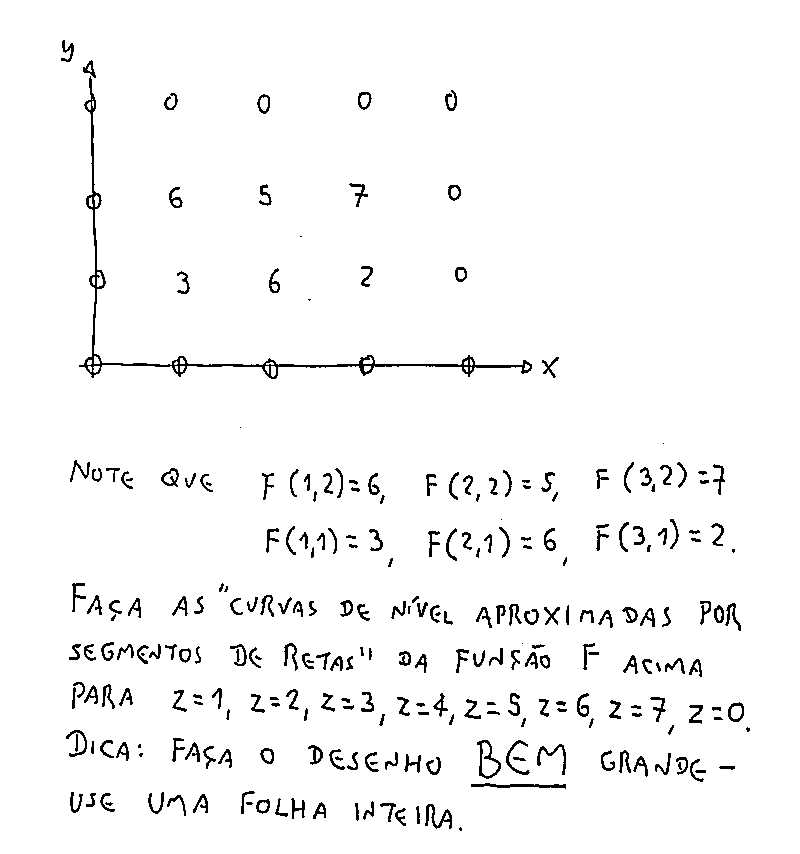
\includegraphics[height=7cm]{2020-2-C3/20210317_curva_de_nivel.pdf}

\newpage

% «exercicio-9-dicas»  (to ".exercicio-9-dicas")

Dica 1:


% (find-latexscan-links "C3" "20210317_curvas_de_nivel_2")
% (find-xpdf-page "~/LATEX/2020-2-C3/20210317_curvas_de_nivel_2.pdf")
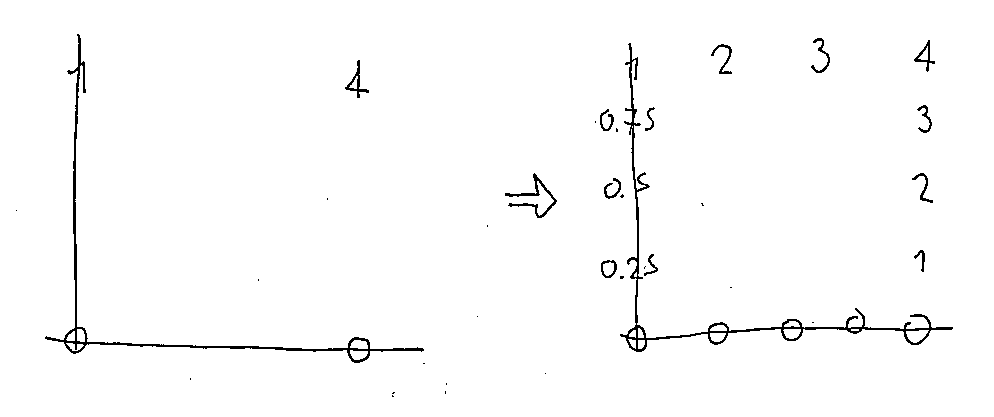
\includegraphics[width=5.5cm]{2020-2-C3/20210317_curvas_de_nivel_2.pdf}

Dica 2:

% (find-latexscan-links "C3" "20210317_curvas_de_nivel_3")
% (find-xpdf-page "~/LATEX/2020-2-C3/20210317_curvas_de_nivel_3.pdf")
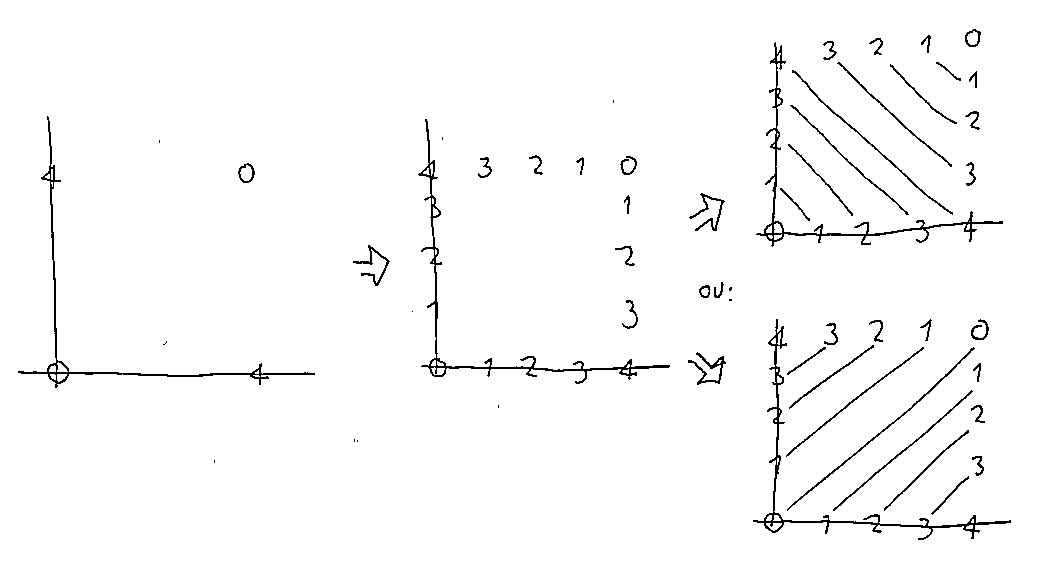
\includegraphics[width=7cm]{2020-2-C3/20210317_curvas_de_nivel_3.pdf}

\newpage

% «dicas-sobre-as-dicas»  (to ".dicas-sobre-as-dicas")
% (c3m202rcadeia1p 20 "dicas-sobre-as-dicas")
% (c3m202rcadeia1a    "dicas-sobre-as-dicas")

{\bf Dicas sobre as dicas (adaptadas da discussão no Telegram)}

Reparem que a gente só sabe o valor de $F(x,y)$ nesses 20 pontos e a
gente vai ter que {\sl tentar} visualizar essa função... por exemplo,
$F(0,0)=0$ e $F(1,0)=0$, né? Então o método do vídeo vai supor que
$F(x,0)$ vai ser 0 em todos os pontos entre $(0,0)$ e $(1,0)$... Deixa
eu mudar o enunciado do exercício. O enunciado novo vai ser...


%  Confere com os das outras pessoas! Tem umas pegadinhas =) Acabei de
% por esse exercicio no PDF. Pus a foto que eu mandei pra voces, mas
% tambem pus uma pagina anterior com algumas explicacoes. mando uma
% foto dela pra voces num instante.

\begin{quote}

  As idéias que eu dei no vídeo dão um método que vai fazer com que
  todo mundo chegue nas mesmas curvas de nível {\sl se vocês decidirem
    juntos o que fazer no caso ambíguo da dica 2}. Eu quero que você
  discutam os detalhes entre vocês até todo mundo chegar a um método
  só e todo mundo obter as mesmas figuras.

\end{quote}

Tem um monte de funções contínuas do retângulo $[0,4]×[0,3]$ em $\R$.
O enunciado do problema diz o valor de $F(x,y)$ em uns poucos
pontos... Em princípio haveriam infinitos jeitos de obter funções $F:
[0,4]×[0,3] → R$ que nos pontos que eu dei valessem os valores que eu
dei... Vocês lembram daqueles problemas de trajetórias em que a gente
sabia $F(t)$ e $F'(t)$ só pra alguns valores de $t$ e a gente ia
tentar reconstruir a trajetória toda de algum jeito razoável a partir
desses pontos? Agora é a mesma coisa, só que pior!... Por exemplo,
naquele exercício de trajetórias voces poderiam começar calculando
$F(0)$, $F'(0)$, $F(\pi/2)$ e $F'(\pi/2)$ porque são pontos em que as
contas são fáceis, mas se vocês quisessem calcular $F(\pi/4)$ e
$F'(\pi/4)$ vocês poderiam usar a calculadora ou o computador e obter
os valores exatos pra esses pontos...

Agora a gente está fazendo algo que parece mais com problemas ``do
mundo real''. É como se vocês tivessem medido a altura da superfície
só em alguns pontos e a partir disso quisessem uma aproximação
razoável pro resto da superfície...

Voces já viram mapas da mundo feitos em 1500 e pouquinho? Em que quem
fez o mapa tinha que fazer uma boa hipótese sobre a forma da América a
partir dos dados das poucas expediçõs que já tinham ido e voltado de
lá? Aqui tem um exemplo --- de 1507, acho:

\ssk

% https://en.wikipedia.org/wiki/Waldseem%C3%BCller_map
\url{https://en.wikipedia.org/wiki/Waldseem\%C3\%BCller_map}

\ssk

Reparem que as Américas do Sul e do Norte são bem magrinhas. Nenhum
europeu sabia como elas eram na direção Oeste, na direção do Oceano
Pacífico e do Japão. O que a gente está tentando fazer agora é mais ou
menos a mesma coisa que isso...

Algumas pessoas --- as que estão acostumadas a encontrar a única
resposta certa --- vão ficar travadas durante horas... por isso é que
eu queria que esse exercicio fosse uma {\sl atividade de grupo} ---
porque acho que algumas outras pessoas vão comecar a discutir os
melhores jeitos de fazer as curvas de nível da função $F(x,y)$, e em
alguns pontos elas vão ter que fazer escolhas em conjunto, e aí em
algum momento as pessoas travadas vao destravar...

Reparem que a gente sabe muito pouco sobre a superfície $z = F(x,y)$.
Pode ser, por exemplo, que ela tenha uma montanha altíssima com pico
no ponto $(0.5,0.5)$, e um vale profundíssimo em $(1.5,0.5)$...

A gente não sabe qual é a função $F(x,y)$ ``de verdade'', e eu quero
ver se vocês conseguem algum desenho pras curvas de nível da $F(x,y)$
que todo mundo ache que é uma aproximação razoável.

Ficou mais claro?


\newpage

Reparem, o Cirillo já estava comecando a fazer curvas de nível do
jeito dele aqui... e eu comentei que o método que eu usei pra fazer as
minhas foi um pouco diferente...

O meu objetivo era que todo mundo discutisse --- Mas acho que eu fiz
algumas pessoas desanimarem com uns comentários que eu fiz



\bsk

Voces acham que entre os dois pontos em que $F(x,y)=6$ tem um segmento
de reta em que $F(x,y)$ é constante $= 6$? Ou não?

{\sl (Umas pessoas acharam que sim, outras que não)}

A figra da dica 2 é sobre isso... aqui a gente vai ter que DECIDIR o que faz.
Tentem fazer dos dois jeitos! Se vocês usarem a opção de cima na ``dica
2'' do slide 19 vocês vão ter um segmento de reta em que $z = 6$ no
segmento todo, e se vocês usarem a opção de baixo os dois `6's vão
virar picos separados...




% Posso gravar se eu entender melhor as duvidas de voces

% Professor, não to entendendo nada
% Tô um pouco perdida tbm
% 
% Professor, o senhor poderia gravar algum vídeo explicando esse exercicio de hoje?
% 
% Não
% Não :(
% 
% 
% Cirillo Moreira C3
% Photo
% Reparem, o Cirillo ja' estava comecando a fazer curvas de nivel do
% jeito dele aqui... e eu comentei que o metodo que eu usei pra fazer as
% minhas foi um pouco diferente
% O meu objetivo era que todo mundo discutisse
% Mas acho que eu fiz algumas pessoas desanimarem com uns comentarios que eu fiz
% 
% GENTE
% Voces podem passar os ultimos 20 minutos de hoje discutindo o exercicio 9?
% A gente vai passar pelo menos metade da aula de sexta discutindo ele tambem, mas por favor comecem hoje...
% Vou colocar no PDF as figuras que eu mandei e uma parte da discussao
% 
% OBAAAAAAA
% Entao agora voces podem discutir os detalhes ate' voces chegarem a
% figuras exatamente iguais =) =) =)
% 
% prof  o z = 7 seria um pico da função?
% Sim!
% 
% Voces fizeram essas figuras com segmentos de retas?
% 
% Eu fiz
% eu fui vendo valores intermediarios e aproximando
% fiz com valores de intermediarios
% partindo de um valor já conhecido
% e aproximando
% 


% Voces acham que entre os dois pontos em que F(x,y)=6 tem um segmento
% de reta em que F(x,y) e' constante = 6? ou nao?
% 
% acho que não
% 
% creio que sim
% 
% Depende. Se a representação for de uma altura constante, sim.
% 
% Essa figura aqui e' sobre isso... aqui a gente vai ter que DECIDIR o que faz
% 
% Acho que pode ter e pode não ter
% 
% Atualizei o PDF:
% http://angg.twu.net/LATEX/2020-2-C3-rcadeia1.pdf
% (Pus as figuras mas ainda nao pus mais texto)
% 
% Tentem fazer dos dois jeitos! Se voces usarem a opcao de cima na "dica
% 2" do slide 19 voces vai ter um segmento de reta em que z = 6 no
% segmento todo, e se voces usarem a opcao de baixo os dois "6"s vao
% virar p icos separados...


% 
% prof a figura seria como uma plano cheio de picos com a altura igual a z ?
% Acho que ela vai ter no maximo 4 picos

%e $(x_0,y_0)=(2,4)$.

% (find-bortolossi5page (+ -161 162) "5. Derivadas parciais")
% (find-bortolossi5page (+ -161 162) "5.1. Lembrando Cálculo 1")
% (find-bortolossi5page (+ -162 164) "5.2. Definições e exemplos")
% (find-bortolossi5page (+ -162 165)   "Fig. 5.2: Interpretação geométrica")

% Aqui a gente pode pensar que $x_0$ e $x_1$ são posições no eixo
% horizontal, $y_0$ e $y_1$ são posições no eixo vertical, $Δx$ é uma
% distância na horizontal, $Δy$ é uma distância na vertical,
% $\frac{Δy}{Δx}$ é uma {\sl inclinação} (qual? Do quê?), e assim por
% diante.

% (c3m201taylor2p 5 "derivacao-implicita")
% (c3m201taylor2    "derivacao-implicita")
% (c3m201taylor3p 2 "na-aula-passada")
% (c3m201taylor3    "na-aula-passada")
% (c3m201sups1p 11 "exercicio-2")
% (c3m201sups1     "exercicio-2")
% (c3m201derpsp 5 "tipos")
% (c3m201derps    "tipos")

\newpage

% «thomas-intro»  (to ".thomas-intro")
% (c3m202rcadeia1p 25 "thomas-intro")
% (c3m202rcadeia1a    "thomas-intro")

{\bf Uma figura do livro do Thomas}

Nos próximos exercícios vocês vão tentar refazer vocês mesmos a figura
do slide 27, que eu roubei do livro ``Calculus - 11th ed.'', do
Thomas/Weir/Hass/Giordano...

...mas vocês vão usar esta função aqui:

$$\begin{array}{rcl}
  G(x,y) &=& 25 - x^2 - y^2 \\ 
  F(x,y) &=& \begin{cases}
             G(x,y)/5 & \text{quando $G(x,y)≥0$}, \\
             0        & \text{quando $G(x,y)<0$} \\
             \end{cases} \\
  \end{array}
$$

...e esta superfícies:

$$\begin{array}{rcl}
   S &=& \setofxyzst{z = F(x,y)} \\
  S' &=& \setofxyzst{x≥0, \; y≥0, \; z = F(x,y)} \\
  \end{array}
$$


\newpage

O diagrama de numerozinhos dela é:

\begin{verbatim}
  0.0 0.0 0.0 0.0 0.0 0.0 0.0 0.0 0.0 0.0 0.0
  0.0 0.0 0.0 1.0 1.6 1.8 1.6 1.0 0.0 0.0 0.0
  0.0 0.0 1.4 2.4 3.0 3.2 3.0 2.4 1.4 0.0 0.0
  0.0 1.0 2.4 3.4 4.0 4.2 4.0 3.4 2.4 1.0 0.0
  0.0 1.6 3.0 4.0 4.6 4.8 4.6 4.0 3.0 1.6 0.0
  0.0 1.8 3.2 4.2 4.8 5.0 4.8 4.2 3.2 1.8 0.0
  0.0 1.6 3.0 4.0 4.6 4.8 4.6 4.0 3.0 1.6 0.0
  0.0 1.0 2.4 3.4 4.0 4.2 4.0 3.4 2.4 1.0 0.0
  0.0 0.0 1.4 2.4 3.0 3.2 3.0 2.4 1.4 0.0 0.0
  0.0 0.0 0.0 1.0 1.6 1.8 1.6 1.0 0.0 0.0 0.0
  0.0 0.0 0.0 0.0 0.0 0.0 0.0 0.0 0.0 0.0 0.0
\end{verbatim}

% G = function (x,y) return 25 - (x*x + y*y) end
% F = function (x,y) if G(x,y) >= 0 then return G(x,y)/5 else return 0 end end
% for y=6,-6,-1 do
%   for x=6,-6,-1 do
%     printf("%4.1f", F(x,y))
%   end
%   print()
% end


\newpage


% «figura-thomas»  (to ".figura-thomas")
% (c3m202rcadeia1p 27 "figura-thomas")
% (c3m202rcadeia1a    "figura-thomas")

% (find-latexscan-links "C3" "2021mar18_thomas_11-1_fig_14.15")
% (find-xpdf-page "~/LATEX/2020-2-C3/2021mar18_thomas_11-1_fig_14.15.pdf")
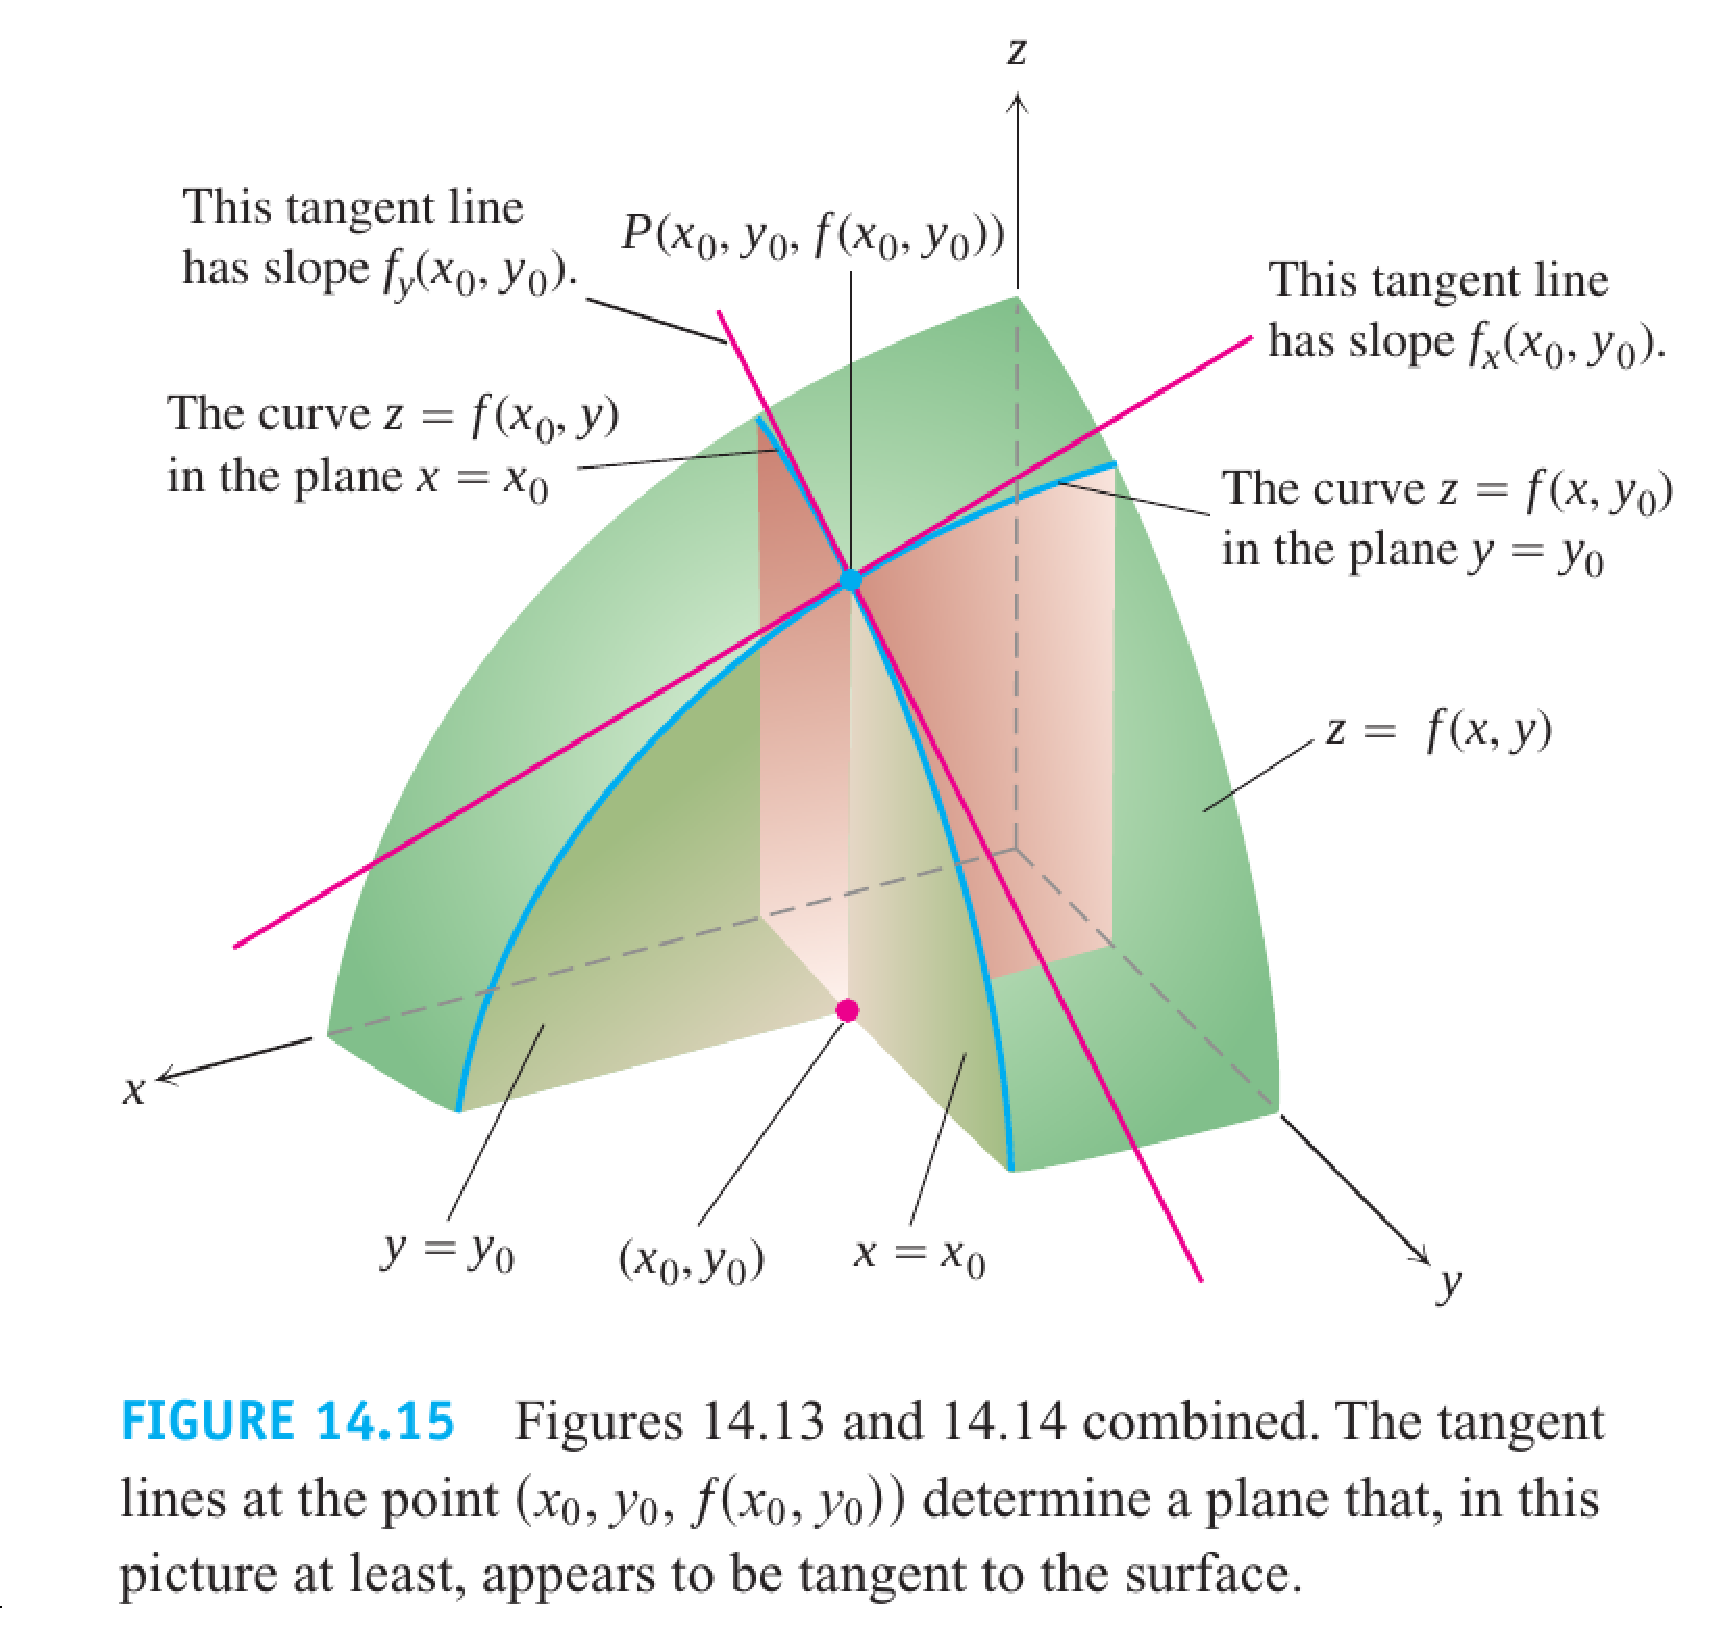
\includegraphics[height=8cm]{2020-2-C3/2021mar18_thomas_11-1_fig_14.15.pdf}

% (find-books "__analysis/__analysis.el" "thomas")
% (find-books "__analysis/__analysis.el" "thomas" "Figure 14.5")


\newpage

% «exercicio-10»  (to ".exercicio-10")
% (c3m202rcadeia1p 28 "exercicio-10")
% (c3m202rcadeia1a    "exercicio-10")

{\bf Exercício 10.}

Aqui vamos usar estas {\sl definições}:

$x_1 = x_0 + Δx$,

$y_1 = y_0 + Δy$,

$z_0 = F(x_0,y_0)$,

$z_1 = F(x_1,y_1)$,

$Δz = z_1 - z_0$,

mas em cada item os valores de $x_0, y_0, Δx, Δy$ vão ser diferentes.

\msk

a) Sejam $x_0=1, y_0=2, Δx=\ColorOrange{-1}, Δy=1$.

{\sl Visualize} as seguintes coisas:

$(x_0,y_0,0)$, $(x_1,y_0,z_0)$, $(x_0,y_1,0)$, $(x_1,y_1,0)$, 

$(x_0,y_0,z_0)$, $(x_1,y_1,z_1)$, $(x_0,y_1,z_0)$, $(x_1,y_0,z_0)$, $(x_1,y_1,z_0)$, 

$(x_0,y_0,z_0) + \VEC{Δx,Δy,Δz}$,

$(x_0,y_0,z_0) + \VEC{Δx,0,\frac{∂z}{∂x}Δx}$,
$(x_0,y_0,z_0) + \VEC{0,Δy,\frac{∂z}{∂y}Δy}$.


\newpage

Dica: algumas pessoas vão querer fazer desenhos em perspectiva, e
outras vão querer calcular tudo numericamente... tudo isso é opcional.
Se você conseguir visualizar todos esses objetos só olhando pro
diagrama de numerozinhos e visualizando a que distância da tela cada
um deles está já tá bom.

\msk

{\bf Exercício 10 (cont.)}

Visualize as seguintes retas parametrizadas:

b) $\setofst{ (x_0,y_0,z_0) + t\VEC{Δx,0,\frac{∂z}{∂x}Δx} }{t∈\R}$,

c) $\setofst{ (x_0,y_0,z_0) + t\VEC{0,Δy,\frac{∂z}{∂y}Δy} }{t∈\R}$,

d) $\setofst{ (x_0,y_0,z_0) + t\VEC{Δx,Δy,\frac{∂z}{∂x}Δx + \frac{∂z}{∂y}Δy} }{t∈\R}$,

e) $\setofst{ (x_0,y_0,z_0) + t\VEC{Δx,Δy,Δz} }{t∈\R}$,

\newpage

{\bf Exercício 10 (cont.)}

Visualize as seguinte curvas parametrizadas:


f) $\setofst{ (x_0, y_0+t, F(x_0,y_0+t)) }{ t∈\R }$,

g) $\setofst{ (x_0, y_0+t, F(x_0,y_0+t)) }{ t∈\R }$,

h) $\setofst{ (x_0+tΔx, y_0+tΔy, F(x_0+tΔx, y_0+tΔy)) }{ t∈\R }$

i) $\setofst{ (x_0+tΔx, y_0, F(x_0+tΔx,y_0)) }{ t∈\R }$,

j) $\setofst{ (x_0, y_0+tΔy, F(x_0,y_0+tΔy)) }{ t∈\R }$,


\bsk


{\bf Exercício 11}

Refaça tudo que você fez no 10, mas mudando o $Δx$ para 0.5.

\bsk

{\bf Exercício 12}

Refaça tudo que você fez no 10 e no 11, mas agora com

$Δx=0.5$ e $Δy=0.5$.


\newpage

% «tipos-de-novo»  (to ".tipos-de-novo")
% (c3m202rcadeia1p 32 "tipos-de-novo")
% (c3m202rcadeia1a    "tipos-de-novo")
% (c3m201derpsp 5 "tipos")
% (c3m201derps    "tipos")

{\bf Tipos (de novo)}

(Adaptado às pressas de slides do semestre passado)

\msk

Dica: {\bf TUDO} que nós estamos fazendo agora pode ser {\sl
  visualizado} e {\sl tipado}. Você já viu um pouco de tipos em {\tt
  C} e em Física; em Física os ``tipos'' são parcialmente determinados
pelas unidades --- metros são distância, segundos são tempo,
metros/segundo é uma unidade de velocidade, e assim por diante...

Aqui a gente pode pensar que $x_0$ e $x_1$ são posições no eixo
horizontal, $y_0$ e $y_1$ são posições no eixo vertical, $Δx$ é uma
distância na horizontal, $Δy$ é uma distância na vertical,
$\frac{Δy}{Δx}$ é uma {\sl inclinação} (qual? Do quê?), e assim por
diante.

\newpage

% «exercicio-13»  (to ".exercicio-13")
% (c3m202rcadeia1p 32 "exercicio-13")
% (c3m202rcadeia1a    "exercicio-13")

{\bf Exercício 13}

Veja se você consegue ``tipar'' (no sentido acima) cada subexpressão
de cada uma das contas que você fez no Exercício 2. Dica: use chaves
sob as subexpressões deste modo aqui,

\def\rq{\ColorRed{?}}
\def\undq#1{\underbrace{#1}_{\rq}}

$$\undq{
  \undq{(\undq{F(\undq{\undq{\undq{x_0} + \undq{Δx}},\undq{y_0}})}
        - \undq{F(\undq{\undq{x_0},\undq{y_0}})})} / \undq{Δx}
  }
$$

e escreva os seus tipos nos lugares em que eu pus as `$\rq$'s. Use
Português onde quiser e improvise o quanto precisar.


\newpage

{\bf Depois do mini-teste}

Na sexta, 19/março/2021, vocês fizeram um mini-teste que pedia pra
vocês desenharem cortes numa figura parecida com a do slide 27...
link:

\ssk

\url{http://angg.twu.net/LATEX/2020-2-C3-MT1.pdf}

\ssk

Agora vocês vão fazer algo bem parecido mas usando a superfície $S'$
do slide 25.

\newpage

% «exercicio-14»  (to ".exercicio-14")

{\bf Exercício 14.}

Desenhe a superfície $S'$ no mesmo ângulo da figura do Thomas

do slide
27 e desenhe sobre ela:

a) $S' ∩ \setofxyzst{z=2}$

b) $S' ∩ \setofxyzst{z=3}$

c) $S' ∩ \setofxyzst{z=4}$

d) $S' ∩ \setofxyzst{x=1}$

e) $S' ∩ \setofxyzst{x=2}$

f) $S' ∩ \setofxyzst{x=3}$


\bsk

% «exercicio-15»  (to ".exercicio-15")
% (c3m202rcadeia1p 34 "exercicio-15")
% (c3m202rcadeia1a    "exercicio-15")

{\bf Exercício 15.}

Faça outras cópias do seu desenho da $S'$ e represente nessas cópias
\ColorRed{\bf \underline{TODOS}} os pontos, retas, curvas e vetores
que você obteve no exercício 10 --- \ColorRed{mas agora use $Δx=-1$}.
Aqui o nosso objetivo é aprender a visualizar em 3D todas essas
construções.

\newpage

\phantom{a}




%\printbibliography

\GenericWarning{Success:}{Success!!!}  % Used by `M-x cv'

\end{document}

%  ____  _             _         
% |  _ \(_)_   ___   _(_)_______ 
% | | | | \ \ / / | | | |_  / _ \
% | |_| | |\ V /| |_| | |/ /  __/
% |____// | \_/  \__,_|_/___\___|
%     |__/                       
%
% «djvuize»  (to ".djvuize")
% (find-LATEXgrep "grep --color -nH --null -e djvuize 2020-1*.tex")

 (eepitch-shell)
 (eepitch-kill)
 (eepitch-shell)
# (find-fline "~/2020.2-C3/")
# (find-fline "~/LATEX/2020-2-C3/")
# (find-fline "~/bin/djvuize")

cd /tmp/
for i in *.jpg; do echo f $(basename $i .jpg); done

convert 2021mar18_thomas_11-1_fig_14.15.png 2021mar18_thomas_11-1_fig_14.15.pdf
f 2021mar18_thomas_11-1_fig_14.15

f () { rm -fv $1.png $1.pdf; djvuize $1.pdf }
f () { rm -fv $1.png $1.pdf; djvuize WHITEBOARDOPTS="-m 1.0" $1.pdf; xpdf $1.pdf }
f () { rm -fv $1.png $1.pdf; djvuize WHITEBOARDOPTS="-m 0.5" $1.pdf; xpdf $1.pdf }
f () { rm -fv $1.png $1.pdf; djvuize WHITEBOARDOPTS="-m 0.25" $1.pdf; xpdf $1.pdf }
f () { cp -fv $1.png $1.pdf       ~/2020.2-C3/
       cp -fv        $1.pdf ~/LATEX/2020-2-C3/
       cat <<%%%
% (find-latexscan-links "C3" "$1")
%%%
}

f 20210317_curva_de_nivel
f 20210317_curvas_de_nivel_2
f 20210317_curvas_de_nivel_3

f 20210226_regra_da_cadeia_1




%  __  __       _        
% |  \/  | __ _| | _____ 
% | |\/| |/ _` | |/ / _ \
% | |  | | (_| |   <  __/
% |_|  |_|\__,_|_|\_\___|
%                        
% <make>

 (eepitch-shell)
 (eepitch-kill)
 (eepitch-shell)
# (find-LATEXfile "2019planar-has-1.mk")
make -f 2019.mk STEM=2020-2-C3-rcadeia1 veryclean
make -f 2019.mk STEM=2020-2-C3-rcadeia1 pdf

% Local Variables:
% coding: utf-8-unix
% ee-tla: "c3m202rcadeia1"
% End:
